%% Para compilar o programa, use pdflatex
%% Opcoes:
%%
%% Cursos:
%% cic: Bacharelado em Ciência da Computação
%% tsi: Técnologo em Sistemas para Internet
\documentclass[tsi]{ifbclass/ifbclass}


\usepackage{listings,xcolor}
\usepackage{inconsolata}

\renewcommand{\lstlistlistingname}{Lista de Algoritmos}
\renewcommand{\lstlistingname}{Algoritmo}

\definecolor{dkgreen}{rgb}{0,.6,0}
\definecolor{dkblue}{rgb}{0,0,.6}
\definecolor{dkyellow}{cmyk}{0,0,.8,.3}

\lstset{
  numbers=left, 
  numberstyle=\small, 
  numbersep=8pt, 
  language        = php,
  basicstyle      = \small\ttfamily,
  keywordstyle    = \color{dkblue},
  stringstyle     = \color{red},
  identifierstyle = \color{dkgreen},
  commentstyle    = \color{gray},
  emph            =[1]{php},
  emphstyle       =[1]\color{black},
  emph            =[2]{if,and,or,else},
  emphstyle       =[2]\color{dkyellow}}



\usepackage{url}


\address{BRASÍLIA}

\title{Sistema de Gerenciamento de Escala de Serviço para o Quartel General do Exército }

\date{2022}

\author{Daniel Evangelista Pereira\\Muller Araújo do Vale}
\adviser{Caio Moura Daoud}

\membroum[a]{Dr.ª Primeira Membro da Banca}
\membrodois{Dr. Segundo Membro da Banca}
\membrotres[a]{Dr.ª Terceira Membro da Banca}
%\membroquatro[a]{Dr.ª Quarta Membro da Banca}

%\coadviser{Nome completo do co-orientador (se existir)} %TODO: nao suportado

% Macros (Se necessario, defina suas proprias aqui)
\def\x{\checkmark}
%\let\lstlistoflistings\origlstoflistings
  \begin{document}

\frontmatter

\frontpage

\presentationpage

% Quando a biblioteca preparar a ficha catalografica, insira-a aqui
% Antes da defesa do trabalho, crie uma ficha falsa
\begin{fichacatalografica}
  \FakeFichaCatalografica
%     \includepdf{fig_ficha_catalografica.pdf} % crie o arquivo come esse nome e descomente essa linha
\end{fichacatalografica}

\banca

%Comente/Remova todo o conteudo entre \begin{dedicatory} e \end{dedicatory} para remover.
\begin{dedicatory} %OPCIONAL
Dedico este trabalho à minha família.
\end{dedicatory}
  
\acknowledgements %OPCIONAL Comente a linha abaixo para remover.
Agradeço ao meu orientador Prof. Dr. Nome do Orientador, pela sabedoria com que me guiou nesta trajetória.

Aos meus colegas de sala.

A Secretaria do Curso, pela cooperação.

Gostaria de deixar registrado também, o meu reconhecimento à minha família, pois acredito que sem o apoio deles seria muito difícil vencer esse desafio. 

Enfim, a todos os que por algum motivo contribuíram para a realização desta pesquisa.


%Novamente, comente todo conteudo entre {epigraph} para remover
\begin{epigraph}[]{Nome do autor} %OPCIONAL
Elemento opcional.

Espaço destinado à epígrafe (elemento opcional). Nesta folha, o autor usa uma citação, seguida de indicação de autoria e ano, relacionada com a matéria tratada no corpo do trabalho.
\end{epigraph}

\resumo
% Escreva seu resumo no arquivo resumo.tex
{\parindent0pt
  SOBRENOME, Prenome do Autor do Trabalho. Título do trabalho: subtítulo (se houver).  2018. 65 f. 
Trabalho de Conclusão de Curso (Graduação) – Tecnólogo em Sistemas para Internet. 
Instituto Federal de Brasília – Campus Brasília. Brasília/DF, 2018.
\vspace{1cm}

Elemento obrigatório, constituído de uma sequência de frases concisas e objetivas,
fornecendo uma visão rápida e clara do conteúdo do estudo. O texto deverá conter no
máximo 500 palavras e ser antecedido pela referência do estudo, com exceção do resumo
inserido no próprio documento. Também, não deve conter citações. O resumo deve ser redigido
em parágrafo único, espaçamento simples e seguido das palavras representativas do conteúdo
do estudo, isto é, palavras-chave, em número de três a cinco, separadas entre si por ponto e
finalizadas também por ponto. Usar o verbo na terceira pessoa do singular, com linguagem
impessoal (pronome SE), bem como fazer uso, preferencialmente, da voz ativa.

\begin{keywords}
Primeira palavra. Segunda palavra. Terceira palavra. Quarta palavra. Quinta-palavra.
\end{keywords}

}
  
\abstract
% Escreva seu abstract em ingles no arquivo abstract.tex
{\parindent0pt
  SOBRENOME, Prenome do Autor do Trabalho. Título do trabalho: subtítulo (se houver).  2018. 65 f. 
Trabalho de Conclusão de Curso (Graduação) – Tecnólogo em Sistemas para Internet. 
Instituto Federal de Brasília – Campus Brasília. Brasília/DF, 2018.
\vspace{1cm}

Elemento obrigatório, constituído de uma sequência de frases concisas e objetivas,
fornecendo uma visão rápida e clara do conteúdo do estudo. O texto deverá conter no
máximo 500 palavras e ser antecedido pela referência do estudo, com exceção do resumo
inserido no próprio documento. Também, não deve conter citações. O resumo deve ser redigido
em parágrafo único, espaçamento simples e seguido das palavras representativas do conteúdo
do estudo, isto é, palavras-chave, em número de três a cinco, separadas entre si por ponto e
finalizadas também por ponto. Usar o verbo na terceira pessoa do singular, com linguagem
impessoal (pronome SE), bem como fazer uso, preferencialmente, da voz ativa.

\begin{keywords}
Keyword. Second keyword. Third keyword. Keyword.
\end{keywords}

}

%ATENCAO.
%Se alguma dessas listas estiver vazia no seu trabalho, comente a linha com um '%'
% Lista de figuras
\listoffigures

% Lista de algortimos
\lstlistoflistings

% Lista de tabelas
\listoftables

% Lista de acronimos
% Acronyms manual: http://linorg.usp.br/CTAN/macros/latex/contrib/acronym/acronym.pdf
\listofacronyms
\begin{acronym}[ACRONYM] 
% Change the word ACRONYM above to change the acronym column width.
% The column width is equals to the width of the word that you put.
% Read the manual about acronym package for more examples:
%   http://linorg.usp.br/CTAN/macros/latex/contrib/acronym/acronym.pdf
\acro{afm}[AFM]{Alphabet Frequency Matrix}
\acro{api}[API]{Application Programming Interface}
\acro{arima}[ARIMA]{Auto-Regressive Integrated Moving Average}
\acro{brn}[BRN]{Bug Report Network}
\acro{bts}[BTS]{Bug Triage System}
\acro{cas}[CAS]{Context-Aware Systems}
\acro{ccb}[CCB]{Change Control Board}
\acro{cr}[CR]{Change Request}
\acro{cvs}[CVS]{Concurrent Version System}
\acro{es}[ES]{Expert System}
\acro{floss}[FLOSS]{Free/Libre Open Source Software}
\acro{glr}[GLR]{Generalized Linear Regression}
\acro{gqm}[GQM]{Goal Question Metric}
\acro{html}[HTML]{HyperText Markup Language}
\acro{ir}[IR]{Information Retrieval}
\acro{irt}[IRT]{Recôncavo Institute of Technology}
\acro{jdt}[JDT]{Jazz Duplicate Finder}
\acro{lda}[LDA]{Latent Dirichlet Allocation}
\acro{loc}[LOC]{Lines of Code}
\acro{lsi}[LSI]{Latent Semantic Indexing}
\acro{ms}[MS]{Mapping Study}
\acro{msr}[MSR]{Mining Software Repositories}
\acro{nlp}[NLP]{Natural Language Processing}
\acro{promise}[PROMISE]{Predictive Models in Software Engineering}
\acro{rbes}[RBES]{Rule-Based Expert System}
\acro{rhel}[RHEL]{RedHat Enterprise Linux}
\acro{saas}[SaaS]{Software as a Service}
\acro{scm}[SCM]{Software Configuration Management}
\acro{serpro}[SERPRO]{Brazilian Federal Organization for Data Processing}
\acro{slr}[SLR]{Stepwise Linear Regression}
\acro{slr}[SLR]{Systematic Literature Review}
\acro{svd}[SVD]{Singular Value Decomposition}
\acro{svm}[SVM]{Support Vector Machine}
\acro{svn}[SVN]{Subversion}
\acro{tfidf}[TF-IDF]{Term Frequency-Inverse Document Frequency}
\acro{vsm}[VSM]{Vector Space Model}
\acro{xp}[XP]{Extreming Programming}
\end{acronym}

% Sumario
\tableofcontents

\mainmatter

%Para cada seção do seu trabalho, edite o arquivo .tex na pasta text/
\chapter{Introdução}
\label{chp:introduction}
Faça aqui, uma introdução geral da área do conhecimento à qual o tema escolhido
está ligado. 

\section{Tema}
A melhor forma de determinar o tema abordado é através de hipóteses. A hipótese
consiste em uma afirmativa que você considera verdadeira e que vai provar ou
buscar provar ao longo de seu trabalho. Outra forma é delimitando o problema em
forma de uma pergunta de partida. Apresente uma visão geral do assunto que será
abordado no trabalho.

\section{Problema}
Dedique este tópico a esclarecer o que o pretende de fato com o seu esforço de
pesquisa. Problema é a questão a ser respondida pelo trabalho, que motivou a sua
realização. É uma questão que já tomou se formou em sua mente, derivada de
teorias da área pesquisada e de sua observação sobre um fenômeno.  Normalmente
se utilizam os subitens abaixo como meios de se determinar claramente os
objetivos, o que também colabora para a delimitação do escopo do trabalho. Está
estreitamente ligado ao objetivo geral, que, normalmente, consiste em encontrar
a resposta para o problema de pesquisa.  O que você viu que é um problema que
precisa de solução? É viável? Você consegue fazer? O problema é sempre uma
dificuldade, uma lacuna.\citep{risg}

\subsection{Objetivo geral}
Desenvolvimento de um sistema web para automação e controle do processo de escala de serviço de militar, possibilitando amenizar as fraudes e falhas humanas.

\subsection{Objetivos específicos}
\begin{itemize}[label=$\bullet$]
    \item Desenvolver um sistema web de escalação automática de militares.
    \item O sistema deve gerar a escala respeitando as normas impostas pelo orgão militar.
    \item O sistema deve notificar os militares que forem escalados.
    \item O sistema deve permitir que os militares corfirmem que estão cientes da escalação.
    \item O sistema deve permitir alterações na escala pelo oficial responsável.
    \item O sistema deve notificar os militares de alterações na escala.
    \item O sistema deve registrar toda e qualquer alteração na escala.
\end{itemize}

\section{Estrutura do TCC}
Neste item você vai descrever como está constituída a monografia, indicando o
que será encontrado em cada uma das sessões seguintes.

\subsection{Classificação da Pesquisa}
Neste item será apresentada a classificação da pesquisa quanto aos objetivos
(exploratória, descritiva ou explicativa); aos procedimentos (Pesquisa
bibliográfica, Pesquisa documental, Pesquisa experimental, Estudo de caso
controle, Levantamento, Estudo de caso ou Estudo de campo) e ao método de
investigação científica (qualitativa ou quantitativa).
 
\chapter{Conceitos Gerais e Revisão da Literatura}
Neste capítulo deve ser proporcionado o estado da arte / referencial teórico
sobre o tema a que se refere o estudo. Um bom pesquisador não deve repetir
trabalhos já concluídos ou que já estão em andamento. Por isso esta sessão é
onde o autor demonstra até onde vai a pesquisa atual no campo de estudos em
questão e estabelece as bases sobre as quais desenvolverá o estudo proposto. A
seguir são mostrados alguns exemplos de como deve-se inserir as figuras e
tabelas. A Figura \ref{fig:exemplo} mostra um exemplo de como inserir uma
figura no texto. A Tabela \ref{tb:exemplo} mostra o exemplo de como uma tabela
deve ser inserida.  Voce pode referenciar capítulos e seções adicionando labels
à elas. Por exemplo, descrevemos a introdução no Capítulo
\ref{chp:introduction}.

\section{Escala de Serviço}
Teste.

\subsection{Eloy}
O programa foi desenvolvido para auxiliar o Sargenteante a escalar os serviços em unidades militares;

Permite montar até 30 escalas que poderão ser definidas pelo próprio operador (Plantão, Gda, Sgt Dia, Of Dia, etc) possibilitando controlar até 500 militares;

O operador pode incluir ou excluir dias na Escala Vermelha ;

As Escalas Vermelhas são montadas ANTES das Pretas (elas são prioritárias) ;

O programa permite que o operador altere as quantidade de postos dos serviços durante a escalação. Isto possibilita: a) a criação de escalas específicas para os dias de meio-expediente (Escala Azul); b) a escalação de serviços cuja responsabilidade da Sub-Unidade ocorra apenas em determinados dias (são aqueles que eventualmente não são escalados TODOS os dias como Cmt Gda e Patrulha); c) que os serviços possam ter número variável de postos ao longo do tempo (0,1,2, etc militares escalados em determinado dia);

Ainda durante os trabalhos de escalação, o operador poderá "forçar" a escalação de um militar em determinado dia e serviço. De forma semelhante, poderá "evitar" que um militar seja escalado em determinado dia e serviço;

A iniciação do Sistema - primeiro uso - é muito facilitada com a guia "Primeira Utilização". Ela orienta o operador na passagem do antigo Sistema (manual) para o novo Sistema (automático).

Com o Módulo de Consultas, o operador poderá obter por exemplo: a quantidade de serviços de cada um dos integrantes das escalas; a relação dos militares que estavam de serviço em determinado dia; a relação de todos os serviços a que determinado militar concorre; a relação dos serviços separadamente nas escalas Vermelha ou Preta; etc);

A realização de Cópias de Segurança é facilmente executada, podendo-se gravar os dados em um "pendrive" para utilização até mesmo em outro computador;

A fotografia e o título existentes na capa do sistema podem ser substituídos pelo nome da Unidade/Subunidade e por uma fotografia livremente escolhida pelo usuário;

O programa possui um Manual "on-line" com as orientações necessárias para que os usuários possam tirar o máximo proveito das facilidades oferecidas pelo Sistema;

O programa procura atender a todas as especificações contidas no RISG ;

Por tratar-se de uma Versão inicial, alguns erros ainda poderão ocorrer, bem como melhorias terão que ser feitas para dar ao Sistema maior funcionalidade. Por essa razão, sugestões e observações serão muito bem-vindas;

O programa roda nas plataformas Windows XP e Vista. Para rodar em Windows 7, 8 e 10 o setup deve ser executando como "administrador" (veja em "Como Instalar");

O desenvolvedor oferece o programa para livre utilização pelas Organizações Militares, estando liberado o download para as mesmas.\citep{eloy}.

\subsection{Planilha Escala Servico Militar Completa}

\begin{table}[htb]
\caption{Características Principais}
\label{tb:exemplo}
\centering
\begin{tabular}{|l|c|r|r|} %left, center, right. Você pode mudar isso
\hline
Desenvolvedor & VASCONEXCEL\\
Nome do software para escritório & Planilha Escala Serviço Militar\\
Modelo & Completo\\
Versão & 1.0 \\
Tempo de licença & 1000 meses \\
Formato	& Digital \\
\hline
\end{tabular}
\end{table}

Planilha de EXCEL criada para auxiliar no controle de efetivo
Controla e gerencia o efetivo de forma simples, intuitiva e objetiva

Funciona somente no EXCEL 2010 em diante (não funciona no LibreOffice)

O arquivo é enviado compactado (.zip) para o email assim que a compra é confirmada.

Especificações da versão COMPLETA:
- Efetivo máximo de 500
- Trabalha com Escalas Internas, Externas, Especiais e Proporcionais
- Cadastra 20 de escalas de cada
- Cadastra 20 destinos diversos
- Cadastra 20 diferentes postos ou graduações
- Gera relatório de previsão das escalas, aditamento, pernoite e mapa da força

Especificações gerais:
- Título principal a critério do usuário
- Imagem da página principal pode ser modificada
- Cor de fundo pode ser alternada em Verde, Azul, Amarelo e Vermelho
- O calendário da escala faz a contagem das escalas em Vermelha, Preta e tem a opção da cor Azul (roxa)

Atenção!
Não é fornecido de maneira alguma a senha para desbloqueio da planilha. Pois se houver modificações da estrutura (simples mudanca de um nome de uma aba ou título de cabeçalhos, excluir ou incluir linhas ou colunas) isso ira interferir diretamente no VBA e comprometer de forma crítica o funcionamento do arquivo.\citep{planilha}

\subsection{Escala de Serviço para Unidades Militares}
Todos os militares estão sujeitos a escalas de serviço e existem várias. Só na casa-mãe de todos os pára-quedistas já estive integrado nas seguintes escalas de serviço, entre outras:

Sentinela à porta de armas e ronda móvel
Cabo auxiliar do comandante da guarda
Sargento de dia à Companhia de Instrução Aeroterrestre
Comandante da Guarda
Largador
Chefe da Área de Embarque
Uma das dificuldades com a nomeação de pessoal para determinada escala, é conseguir escalar o pessoal de forma justa, usando critérios uniformes com uma boa dose de bom senso e ginástica mental. Para ajudar nesta tarefa, desenvolvi uma aplicação para acompanhar o escalador a melhor nomear o pessoal.

A folha de apresentação do programa. É possível configurar uma escala de serviço até 10 militares (para a mesma escala).

\begin{figure}[!htb]
    \centering
    \caption{Tela Ínicial da Planilha}
    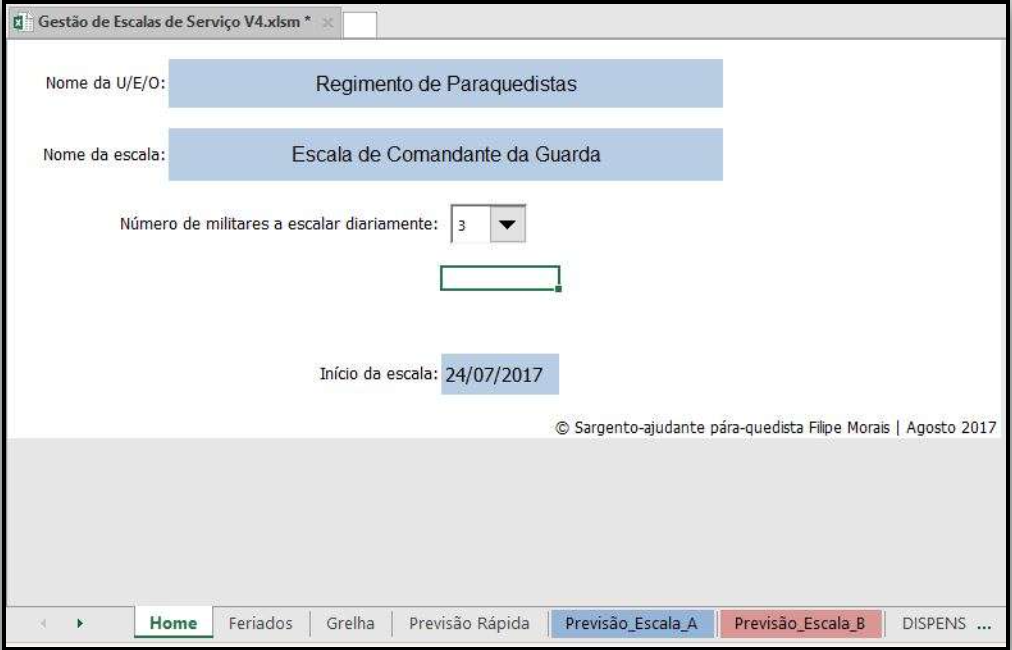
\includegraphics[width=0.35\textwidth]{images/04 - ESUM.png}

    {\footnotesize Fonte: Página oficial do Programa\protect\footnotemark}
    \label{fig:arduino_uno}
\end{figure}

Na grande maioria dos serviços militares existem dois tipos de escala:

A escala A - definida para os dias de semana;

A escala B - definida para os feriados e fins-de-semana.

Assim e por forma a que o programa reconheça os feriados, é necessário introduzi-los no mesmo.

\begin{figure}[!htb]
    \centering
    \caption{Tela de Fériado}
    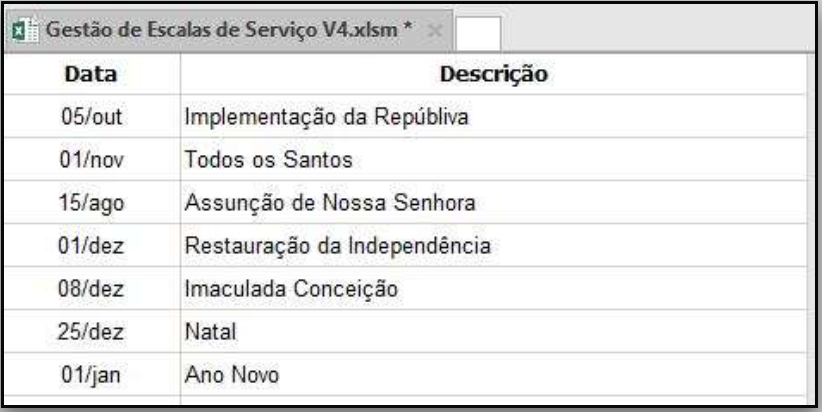
\includegraphics[width=0.35\textwidth]{images/03 - ESUM.png}

    {\footnotesize Fonte: Página oficial do Programa\protect\footnotemark}
    \label{fig:arduino_uno}
\end{figure}

O programa permite obter uma visualização imediata dos próximos a fazer serviço ou seja, uma lista ordenada por ordem dos mais folgados na escala.


\begin{figure}[!htb]
    \centering
    \caption{Tela dos Militeres Escalado}
    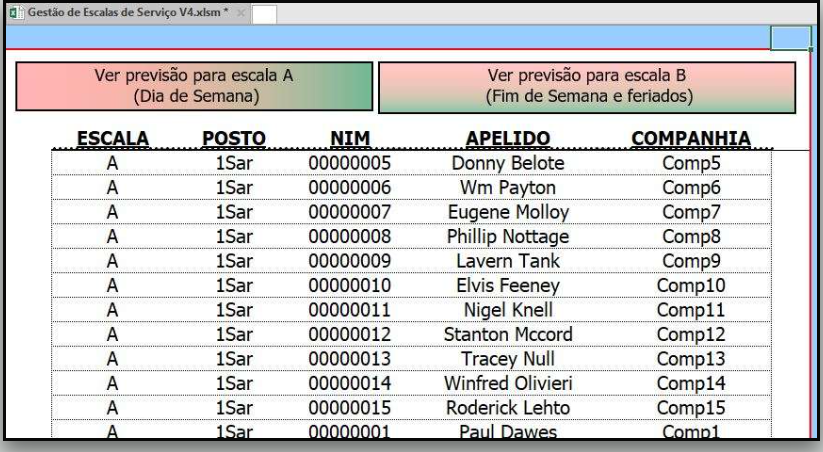
\includegraphics[width=0.35\textwidth]{images/02 - ESUM.png}

    {\footnotesize Fonte: Página oficial do Programa\protect\footnotemark}
    \label{fig:arduino_uno}
\end{figure}


O programa permite imprimir uma previsão da escala. Isto permite aos militares integrados na mesma uma maior coordenação e planeamento da vida pessoal com a profissional.

\begin{figure}[!htb]
    \centering
    \caption{Tela de Impressão}
    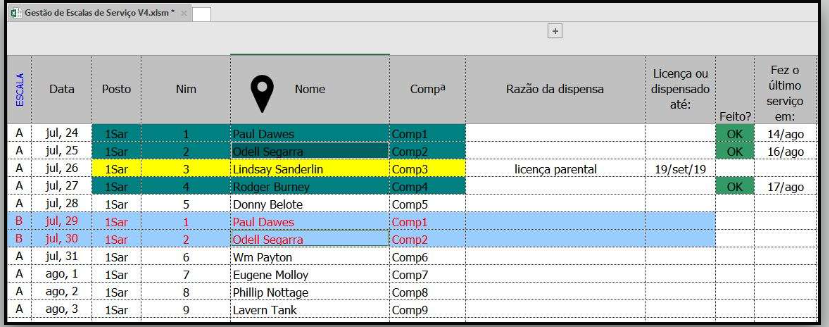
\includegraphics[width=0.35\textwidth]{images/01 - ESUM.png}

    {\footnotesize Fonte: Página oficial do Programa\protect\footnotemark}
    \label{fig:arduino_uno}
\end{figure}

Esta folha é a mais importante do programa. É aqui que vão sendo inseridos os militares conforme vão concluindo o serviço e os próximos a fazer o mesmo.

A forma de o fazer está explicada em detalhe no vídeo, mais abaixo nesta página.

\begin{figure}[!htb]
    \centering
    \caption{Tela dos Militeres Escalado}
    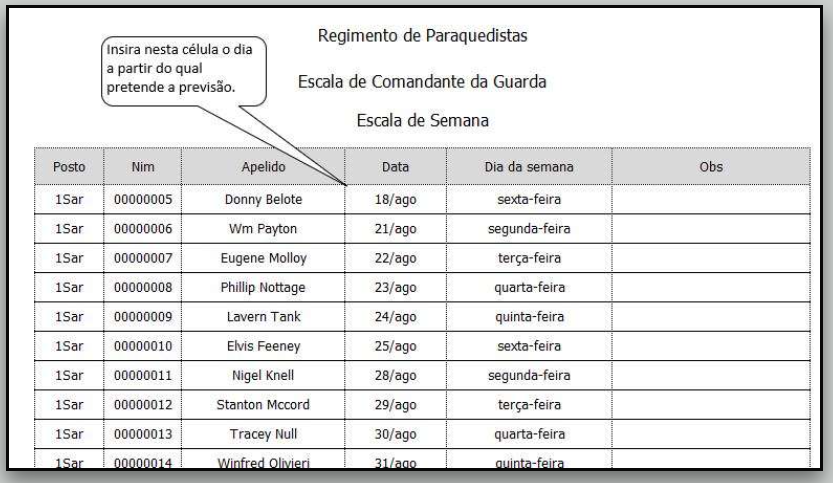
\includegraphics[width=0.35\textwidth]{images/00 - ESUM.png}

    {\footnotesize Fonte: Página oficial do Programa\protect\footnotemark}
    \label{fig:arduino_uno}
\end{figure}

\section{Tecnologias}
Esse capítulo apresenta as tecnologias usadas no desenvolvimento do sistema. Como linguagem de programação, foi utilizado o PHP, acessado via servidor Nginx, com o auxílio do framework Laravel. Para a base de dados, foi utilizado sistema de gerenciador de banco de dados MariaDB. Para orquestrar todos os serviços necessários para subir a aplicação, foi utilizado o Docker.

\subsection{PHP}
Desde sua criação em 1994, a linguagem PHP (Hypertext Preprocessor ou preprocessador de hypertexto, no português), vem sendo amplamente utilizada na web. Mais de 70\% dos sites da web usam PHP no lado do servidor \citep{w3techs}.

A linguagem PHP permite que se trabalhe tanto com servidores windows como servidores linux, a sua evolução permititu que a linguagem abordasse paradigmas estruturados e orientadado a objetos, e comporta diversos bancos de dados, e vem recebendo atualizações constantes, sendo uma lingugem que pode ser tranquilamente utilizada em novos projetos \citep{phpdocs}.
    
\subsection{Laravel}
Laravel é um framework que traz consigo diversas funcionalidades através das suas bibliotecas consolidadas, que vem agregadas ao seu núcleo. Lançado sua primeira versão em 2011, hoje se encontra na versão 9, acompanhando e explorando as novas funcioncionalidades das versões mais atuais do php \citep{laradocs}.
    
O framework hoje conta com 70 mil estrelas no github, o que indica que é um framework bastante conhecido e consolidado no mercado. Atende tanto pequenos quanto grandes projetos, sempre utilizando os padrões mais modernos da linguagem \citep{lararepo}
        
\subsection{Laravel Auditing}
Laravel Auditing, é uma biblitoeca feito para o laravel framework, com o intuito de permitir salvar as mudanças e alterações executadas nas classes de modelo do laravel. Sua configuração padrão permite que registre e recupere os históricos de alterações a partir de uma base de dados, mas também permite que realize a integração com outros meios de logs, como salvar em arquivos ou criar seu próprio driver, para atender a uma necessidade específica \citep{auditdocs}.
    

\subsection{MariaDB}
MariaDB é um sistema gerenciador de banco de dados relacional, que está a mais de 20 anos no mercado.  Sendo um software de codigo aberto, recebe contantes contribuições de comunidades de desenvolvedores que o utilizam, inclusive patches de segurança, tendo esse como um dos principais motivos para utilizá-lo no projeto \citep{mariadbdocs}.
    
\subsection{Nginx}
Escrito por Igor Sysoev, o Nginx é um servidor de proxy reverso HTTP, proxy de servidor de e-mail e um proxy generico de TCP/UDP. Uma de suas características é a possibilidade de configurá-lo em servidores distintos, suportando servidores tanto windows como linux \citep{nginxdocs}.

Oferece um alto desempenho de conexões, sendo seu uso recomendável para aplicações que exigem muitas requisiçoes, ou seja, é escalável e de código aberto.
    
\subsection{Docker}

Docker, tecnologia que divide a aplicação em pequenos containers, tendo cada uma a sua configuração, distinta umas das outras. Permite a entrega rápida de software, e a reprodução do mesmo ambinte tanto pra desenvolvimento quanto homologação e produção \citep{dockerdocs}. 


%\lipsum[2-15]

\let\cleardoublepage\clearpage
\chapter{Metodologia}

Aqui conterão os métodos e procedimentos adotados no desenvolvimento do
trabalho. Esta é uma das sessões mais importantes pois demonstra o poder
científico que foi utilizado para a pesquisa. Sem uma boa metodologia a
pesquisa pode perder a validade. O pesquisador deve utilizar métodos ou
técnicas aceitas pela comunidade científica na busca de provar suas hipóteses.

A metodologia escolhida deve ser aquela que mais se adéqua ao seu objeto de
estudo e à abordagem aplicada. Há dois métodos principais: 1) quantitativo, que
é o uso de instrumental estatístico, de dados numéricos; e 2) qualitativo, que
se caracteriza pela qualificação dos dados coletados, durante a análise do
problema.

\section{Uma seção}
Texto.

\section{Arquitetura}

\chapter{Apresentação e Análise dos Resultados}
O objeto deste trabalho é um sistema que faz o gerenciamento e a escalação automática de militares. O presente capítulo busca apresentar as funcionalidades implementadas no sistema e os passos necessários para realizar o build da aplicação.

\section{Sistema}

O sistema foi desevolvido utilizando o método de containerização, ou seja cada serviço tem o seu container. Para se construir a aplicação é necessário clonar o repositório, disponível \url{https://github.com/daniboyBr/tcc-escala-permanencia-v2}, e seguir os passos descritos no arquivo README.md. Após seguir todos os passos o sistema pode ser acesso em \url{http://localhost:8080}. Para se testar a aplicação, a base de dados foi populada com dados fictícios, podendo o perfil de administrador ser acessado com o e-mail "admin@permanencia.com" e a senha "123456789".

\subsection{Acessando o sistema}

A página inicial do sistema exibe o formulário de login, apresentada na \ref{fig:login}, é por meio dele que todo militar terá acessso as funcionalidades, sendo que algumas delas só é acessível para o usuário administrador do sistema.

\begin{figure}[!htb]
    \centering
    \caption{Tela de Login}
    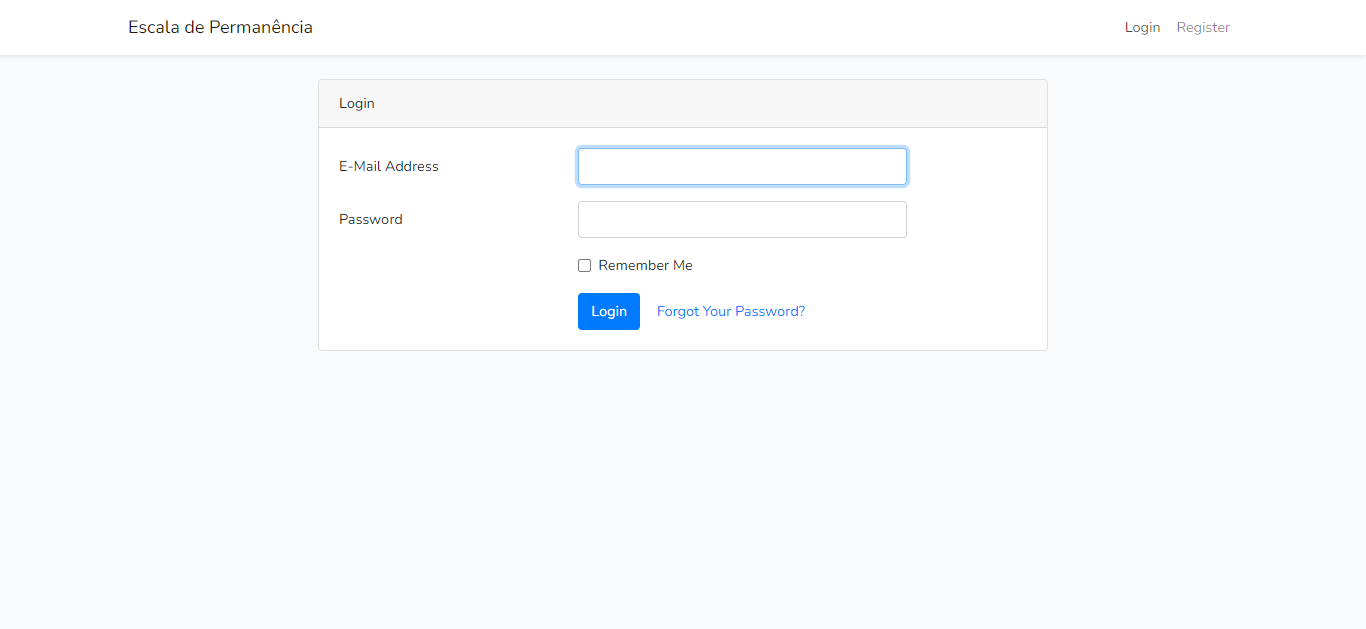
\includegraphics[width=0.8\textwidth]{images/1 - Pagina Inicial - Tela de Login.png}
    \label{fig:login}
\end{figure}

\subsection{Registrando-se no Sistema}

Na Figura \ref{fig:singnup} é mostrada a tela em que o militar deve realizar o seu cadastro, sendo que os campos e-mail e identidade devem ser únicos para cada militar.

\begin{figure}[!htb]
    \centering
    \caption{Tela de Cadastro de Militar}
    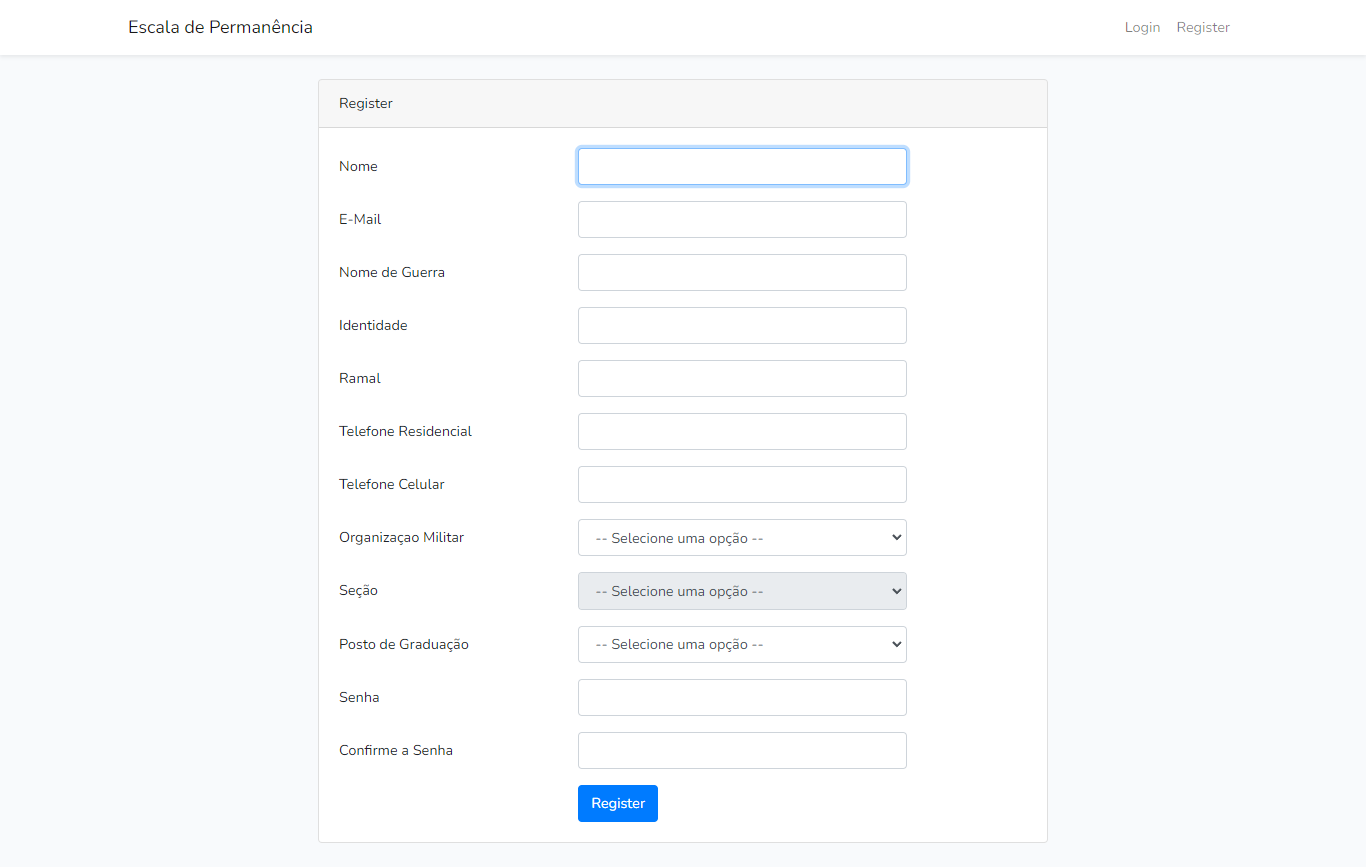
\includegraphics[width=0.8\textwidth]{images/2 - Tela de Cadastro.png}
    \label{fig:singnup}
\end{figure}

O militar, após ter efetuado cadastro, consegue ter acesso ao sistema, porém seu cadatro permanece inativo até que um usuário com perfil de administrador ativar seu cadastro, conforme apresentado na Figura \ref{fig:userinative}

\begin{figure}[!htb]
    \centering
    \caption{Tela de Militar Inativo}
    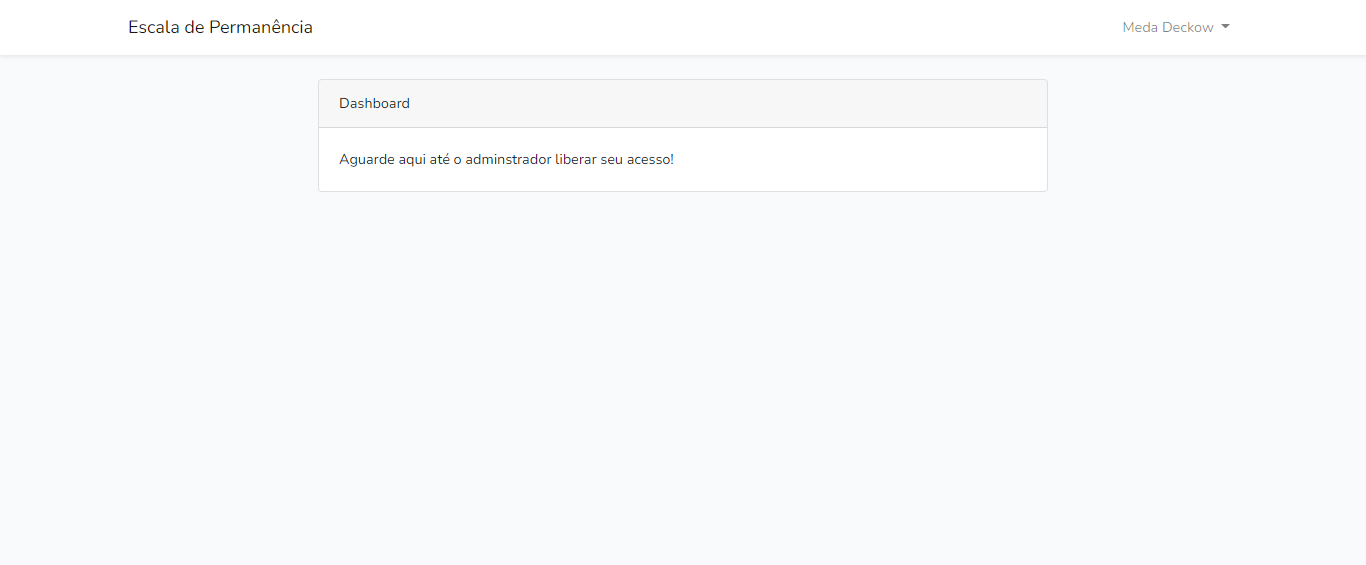
\includegraphics[width=0.8\textwidth]{images/3 - Tela de Militar Inativo.png}
    \label{fig:userinative}
\end{figure}

\subsection{Escala de Serviço}

Ao ter acesso ao sistema, com o cadastro ativo, o militar consegue visualizar a escala do dia corrente, tendo a possibilidade de pesquisar a escalação em datas futuras ou passadas por meio do filtro de data, conforme, apresentado na Figura \ref{fig:escalaservico}.

\begin{figure}[!htb]
    \centering
    \caption{Tela da Escala de Serviço}
    \includegraphics[width=0.8\textwidth]{images/4 - Tela de Visualizacao da Escala de Serviço.png}
    \label{fig:escalaservico}
\end{figure}

Na Figura \ref{fig:escalaservico}, é mostrado o botão livro, é através desse botão que o militar, no dia da sua escalação ao acessar o sistema, consegue relatar toda e qualquer ocorrência após o término do serviço, esse relato pode ser preechido no formulário apresentado na Figura \ref{fig:livroregistro}, uma vez registrado não se pode mais alterar a ocorrência informada.

\begin{figure}[!htb]
    \centering
    \caption{Tela Livro de Registro}
    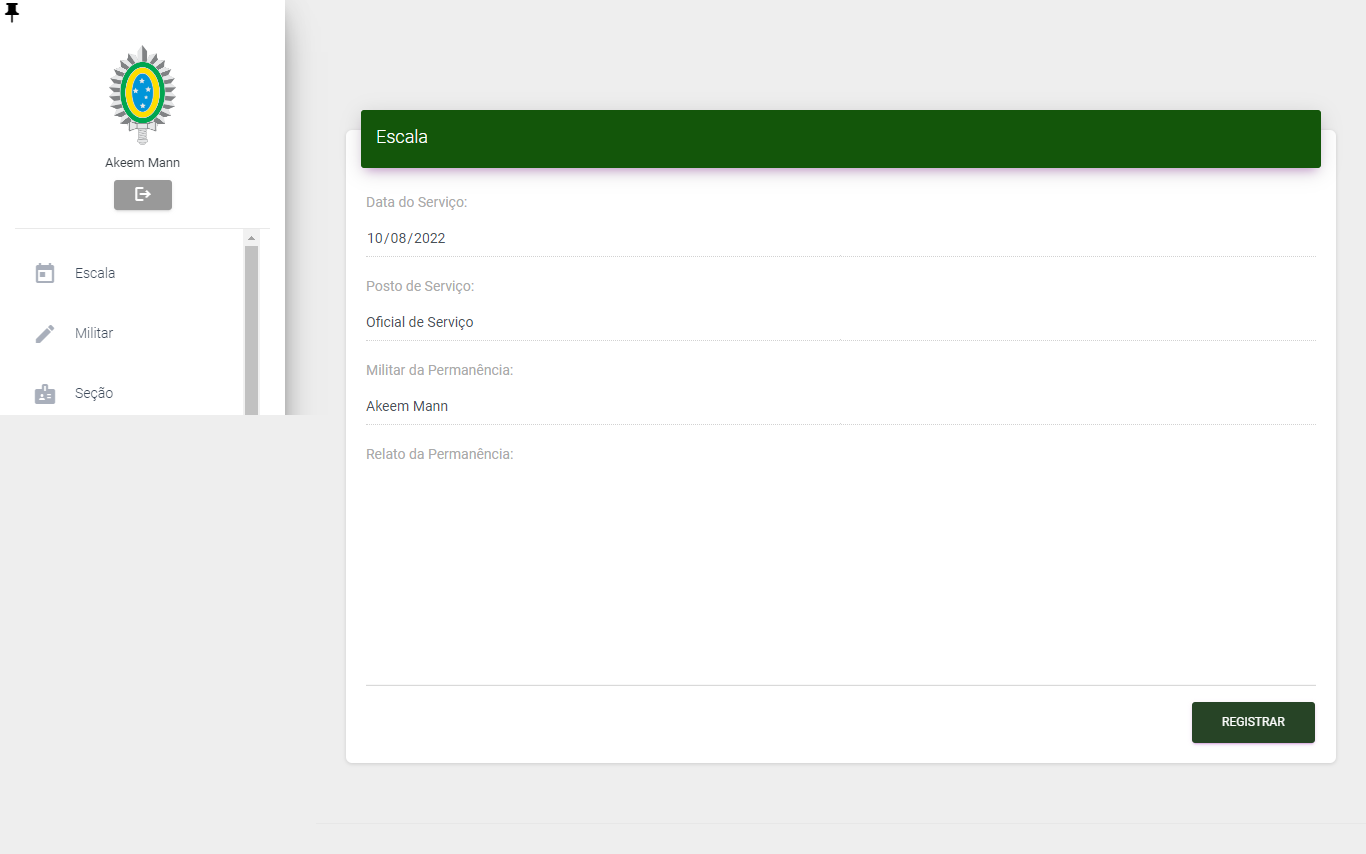
\includegraphics[width=0.8\textwidth]{images/5 - Tela Livo de Registro.png}
    \label{fig:livroregistro}
\end{figure}


\subsection{Escalação Automática de Militares}

A geração da escala acontece por debaixo dos panos. O Laravel disponibiliza uma classe chamada Command, a qual é necessário extender para criar um comando personalizado. Ao extender essa classe, foi implementadao o método handle, responsável por conter toda lógica para escalar e regras para escalar os militares,  conforme apresentado no Algorítimo \ref{lst:algofirst}.

\begin{center}
\noindent\begin{minipage}[t]{0.80\linewidth}
\begin{lstlisting}[frame=single, caption={Classe responsável por gerar escala}, label={lst:algofirst}]
class DailyScale extends Command
{
    protected $signature = 'scale:daily';
    /**  ommited code  */
    public function handle()
    {
        /**  logic to generate scale  */
    }
}
\end{lstlisting}
\end{minipage}
\end{center}

Ao se criar um comando personalizado no laravel, o mesmo ainda não é disparado de imediato, foi necessário configurá-lo na classe Kernel que extende de ConsoleKernel, para isso obrigatoriamente devemos informar um comando e a frequência na função schedule, conforme mostrado no Algorítmo \ref{lst:algosecond}. A escalação automática foi está para rodar todo dia a meia-noite.

\begin{center}
\noindent\begin{minipage}[t]{0.80\linewidth}
\begin{lstlisting}[frame=single, caption={Configuração da geração da escala}, label={lst:algosecond}]
class Kernel extends ConsoleKernel
{
    protected $commands = [
        DailyScale::class
    ];
    protected function schedule(Schedule $schedule)
    {
        $schedule->command('scale:daily')->daily();
    }
    /**  ommited code  */
}
\end{lstlisting}
\end{minipage}
\end{center}

\subsection{Notificação de Militares}

Quando a escala é gerada, um e-mail é enviado para o militar, no e-mail que ele cadastrou no sistema, conforme a Figura \ref{fig:notification}. Esse mesmo e-mail possui um link de confirmação, que ao ser clicado confirma que o militar esta ciente de sua escalação.

\begin{figure}[H]
    \centering
    \caption{Notificação do Militar}
    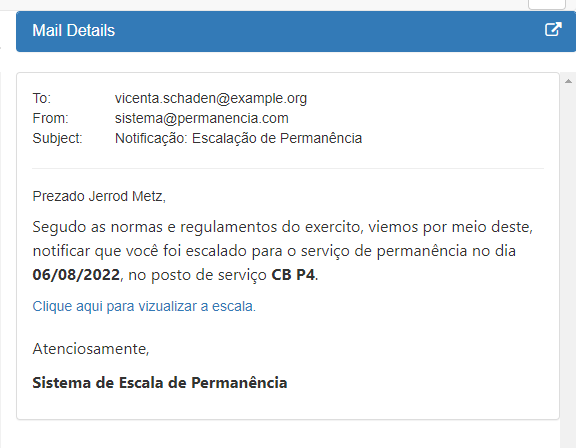
\includegraphics[width=0.8\textwidth]{images/6 - Email enviado.png}
    \label{fig:notification}
\end{figure}

Na Figura \ref{fig:notificationreplace}, mostra o e-mail enviado ao militar caso haja alguma alteração na escala, o mesmo também deve confirmar que está ciente de que houve uma troca na escala e ambos os militares são notificados, o que estava escala antes da troca e o militar que vai realizar a troca.

\begin{figure}[H]
    \centering
    \caption{Notificação de Troca de Militar}
    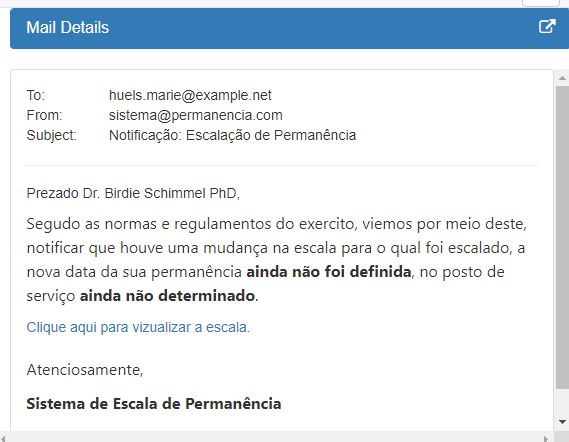
\includegraphics[width=0.8\textwidth]{images/6 - Email enviado Troca.png}
    \label{fig:notificationreplace}
\end{figure}

\subsection{Troca de Militares}

O usuário adminstrador ou escalante, só pode executar uma ação na escala, que é a troca de militares. A troca de militaress só é possível se a escala não estiver fechada, ou seja, se a escala não for da data corrente ou se já passou da data do serviço. Quando a troca de militar está habilitada aparece o botão trocar, conforme apresentado na  Figura \ref{fig:replace}.

\begin{figure}[!htb]
    \centering
    \caption{Troca de Militar}
    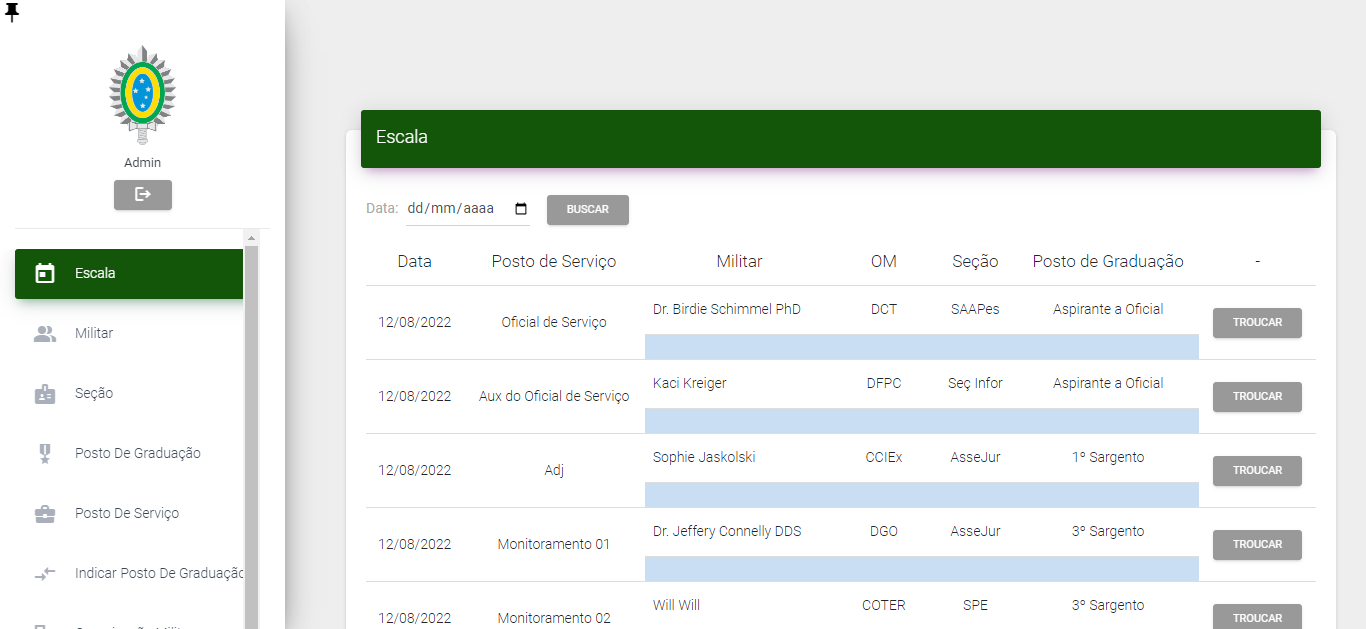
\includegraphics[width=0.8\textwidth]{images/7 - Troca de Militar.png}
    \label{fig:replace}
\end{figure}

Quando clicado no botão de troca o administrador é redirecionado pra uma página que contém o formúlario para efetuar a troca. Primeiro é  necessário buscar o militar que vai substituir o militar escalado, para isso é preciso informar a identidade do militar, conforme a Figura \ref{fig:formreplace}.

\begin{figure}[!htb]
    \centering
    \caption{Formulário para Troca de Militar}
    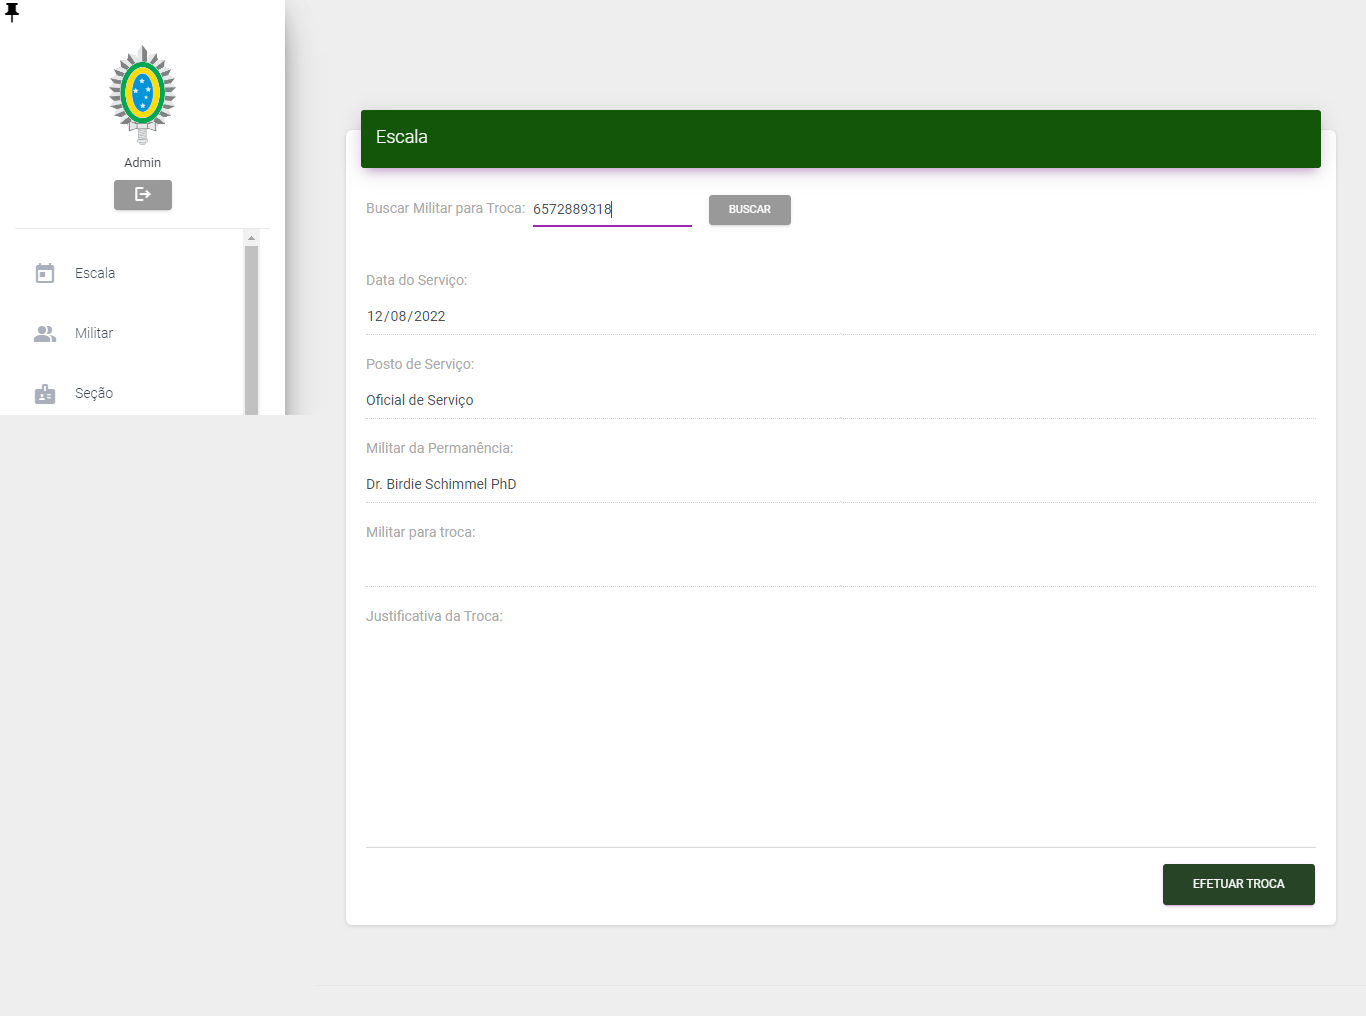
\includegraphics[width=0.8\textwidth]{images/7 - Troca de Militar - 2.png}
    \label{fig:formreplace}
\end{figure}

Para efetivar a troca, o militar que irá substituir o militar escalado deve possuir a mesma grauação configurarada para aquele serviço, senão será apresentada a mensagem demonstrada na Figura \ref{fig:formreplaceerror}.

\begin{figure}[!htb]
    \centering
    \caption{Formulário para Troca de Militar}
    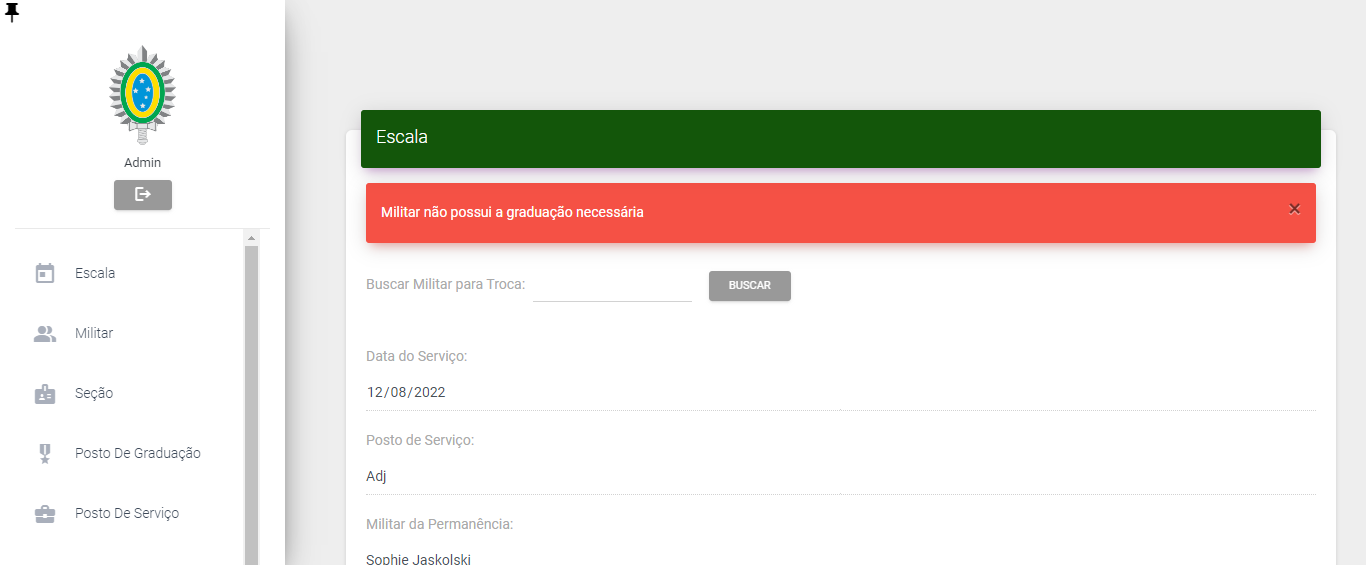
\includegraphics[width=0.8\textwidth]{images/7 - Erro Troca de Militar - Graduação.png}
    \label{fig:formreplaceerror}
\end{figure}

A Figura \ref{fig:formreplaceerror2} também demonstra um outro erro que pode ocorrer caso o administrador tente cadastrar um militar que estaja impedido naquela data.

\begin{figure}[!htb]
    \centering
    \caption{Formulário para Troca de Militar}
    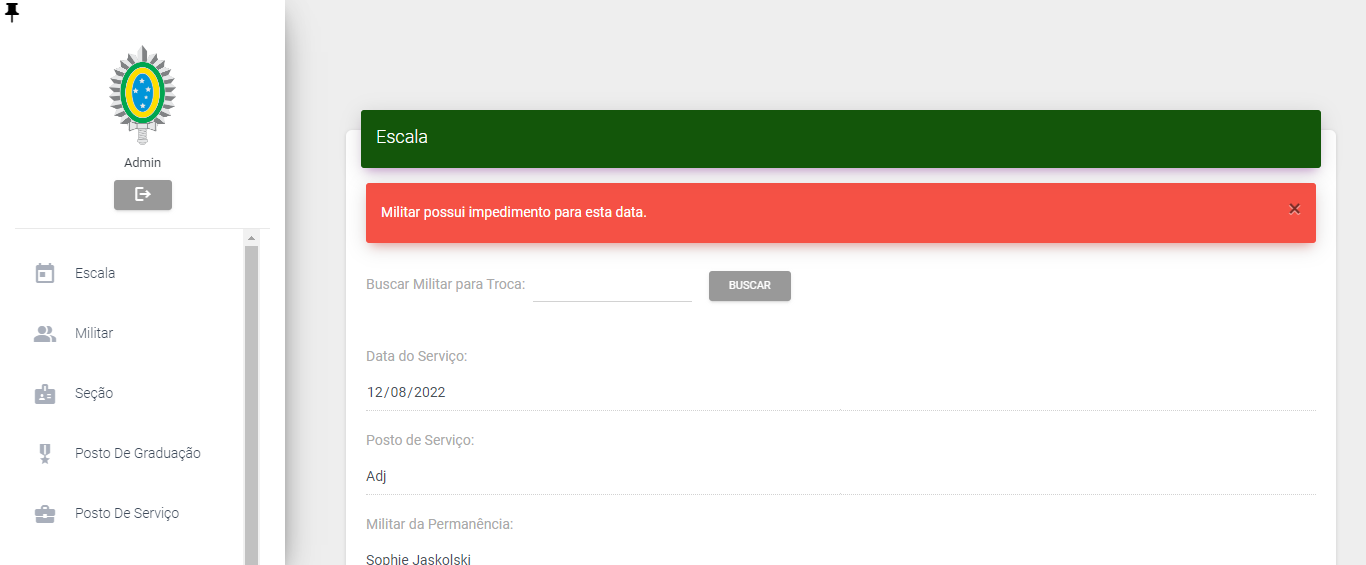
\includegraphics[width=0.8\textwidth]{images/7 - Erro Troca de Militar - Impedimento.png}
    \label{fig:formreplaceerror2}
\end{figure}

Seguindo essas duas regras, o militar a ser escalado possuir a graduação necessária e não estar em impedimento e informando uma justificativa, a troca é realizada com sucesso, conforme demonstrado na Figura \ref{fig:formreplacesuccess}.

\begin{figure}[H]
    \centering
    \caption{Escala após Troca}
    \includegraphics[width=0.8\textwidth]{images/7 - Escala após a Troca de Militar.png}
    \label{fig:formreplacesuccess}
\end{figure}

\chapter{Conclusões e Trabalhos Futuros}

Ao se o observar o problema de escalar equitativamente militares para determinados serviços, e as inúmeras falhas e fraudes geradas nesse processo, viu-se a necessidade de implementar um sistema que automatize o processo de escalação de militares e possibilitasse a auditoria em casos de suspeita de fraude. 

Desenvolvido utilizando tecnologias como PHP e Laravel framework, o sistema pode ser rapidamente desenvolvido e implementado. Devido a sua vasta documentação e inúmeras bibliotecas dispónivel, pode ainda ser expandido e facilmente mantido. O sistema desenvolvido está em sua versão beta e compreende os requisitos mínimos para a solução do problema, que é a escalação equitativa de militares e a rastreabilidade das modificações 
Com a adesão do sistema, passa-se a ter os dados centralizados e disponíveis a qualquer instante, além da rastreabilidade das modificações.

O mesmo  sistema pode ser aderido por outras áreas além do Quartel General do Exécito, mas para isso é necessário implementar as regras específicas daquele setor.

Uma outra modificação que seria benéfica e recomendável, em uma versão futura, é a separação dos dados referentes a auditoria de dados do sistema. Isso se faz necessário pois conforme o tempo passa pode se ter um volume maior de dados de auditoria do que de informações do sistema. Uma possibilidade é transferir os dados referentes a auditoria para um serviço próprio pra isso como servidores de logs, a exemplo o Graylog, que é um software livre capaz de indexar a informação permitindo buscas mais otimizadas e possui base de dados independente. Essa melhoria aumentaria ainda mais a segurança pois retiraria qualquer possibilidade de modificação dos dados por parte de pessoas que fazem manutenção do sistema.




% Referencias

\begin{references}
  \bibliography{bib/references}
\end{references}

% Apendice

\theappendix
\chapter{Mapping Study's Instruments}
\label{ap:mapping-study}

\begin{table}[!htp]
	\centering
	\caption{List of conferences on which the searches were performed.}
	\label{tbl:conferences_list}
	\rowcolors{2}{lightgray!30}{white}
	\resizebox{\columnwidth}{!}{
	\begin{tabular}{ll}
	\toprule
	\textbf{Acronym} & \textbf{Conference} \\
	\toprule
	APSEC & Asia Pacific Software Engineering Conference \\
	ASE   & IEEE/ACM International Conference on Automated Software Engineering \\
	CSMR  & European Conference on Software Maintenance and Reengineering \\
	ESEC  & European Software Engineering Conference \\
	ESEM  & International Symposium on Empirical Software Management and Measurement \\
	ICSE  & International Conference on Software Engineering \\
	ICSM  & International Conference on Software Maintenance \\
	ICST & International Conference on Software Testing \\
	InfoVis & IEEE Information Visualization Conference \\
	KDD   & ACM SIGKDD International Conference on Knowledge Discovery and Data Mining \\
	MSR   & Working Conference on Mining Software Repositories \\
	OOPSLA & Object-Oriented Programming, Systems, Languages and Applications \\
	QSIC  & International Conference On Quality Software \\
	SAC & ACM Symposium on Applied Computing \\
	SEAA & EUROMICRO Conference on Software Engineering and Advanced Applications\\
	SEDE & 19th International Conference on Software Engineering and Data Engineering \\
	SEKE  & International Conference on Software Engineering and Knowledge Engineering \\
	\bottomrule
	\end{tabular}
	}
\end{table}

\begin{table}[htp]
	\caption{List of journals in which the searches were performed.}
	\label{tbl:journals_list}
	\centering
	\rowcolors{2}{lightgray!30}{white}
	\begin{tabular}{l}
	\toprule
	\textbf{Journal title} \\
	\toprule
	ACM Transactions on Software Engineering and Methodology \\
	Automated Software Engineering \\
	Elsevier Information and Software Technology \\
	Elsevier Journal of Systems and Software \\
	Empirical Software Engineering \\
	IEEE Software \\
	IEEE Computer \\
	IEEE Transactions on Software Engineering \\
	International Journal of Software Engineering and Knowledge Engineering \\
	Journal of Software: Evolution and Process \\
	Software Quality Journal \\
	Journal of Software \\
	Software Practice and Experience Journal \\
	\bottomrule
	\end{tabular}
\end{table}

\begin{table}[h]
\centering
\footnotesize
 \rowcolors{2}{lightgray!30}{white}
\caption{Search string per Search Engine.}
\label{tbl:stringengine}
\begin{tabular}{p{.15\textwidth}p{.8\textwidth}}
\toprule
\textbf{Search Engine} & \textbf{Search String}\\
\toprule
   	 	Google Scholar &  bug report OR track OR triage ``change
   	 	request'' issue track OR request OR software OR ``modification request'' OR
   	 	``defect track'' OR ``software issue''  repositories maintenance evolution\\

   	 	ACM Portal & Abstract: "bug report" or Abstract:"change request"
   	 	or Abstract:"bug track" or Abstract:"issue track" or  Abstract:"defect
   	 	track" or Abstract:"bug triage" or Abstract: "software issue" or Abstract: "issue request"
   	 	or Abstract: "modification request") and  (Abstract:software or
   	 	Abstract:maintenance or Abstract:repositories or Abstract:repository \\

   	 	IEEExplorer (1) & (((((((((("Abstract": "bug report") OR
   	 	"Abstract":"change request") OR "Abstract":"bug track") OR "Abstract":"software issue") OR "Abstract":"issue request") OR
        "Abstract":"modification request") OR "Abstract":"issue track") OR
	    "Abstract":"defect track") OR "Abstract":"bug triage") AND
	    "Abstract":software)\\

         IEEExplorer (2) & (((((((((("Abstract": "bug report") OR
         "Abstract":"change request") OR "Abstract":"bug track") OR "Abstract":"software issue") OR
         "Abstract":"issue request") OR "Abstract":"modification request") OR
         "Abstract":"issue track") OR "Abstract":"defect track") OR
         "Abstract":"bug triage") AND "Abstract":maintenance)\\

         IEEExplorer (3) & (((((((((("Abstract": "bug report") OR
         "Abstract":"change request") OR "Abstract":"bug track") OR "Abstract":"software issue") OR
         "Abstract":"issue request") OR "Abstract":"modification request") OR
         "Abstract":"issue track") OR "Abstract":"defect track") OR
         "Abstract":"bug triage") AND "Abstract":repositories)\\

         IEEExplorer & (((((((((("Abstract": "bug report") OR
         "Abstract":"change request") OR "Abstract":"bug track") OR "Abstract":"software issue") OR
         "Abstract":"issue request") OR "Abstract":"modification request") OR
         "Abstract":"issue track") OR "Abstract":"defect track") OR
         "Abstract":"bug triage") AND "Abstract": repository)\\

         Citeseer Library & (abstract: "bug report" OR abstract:"change request" OR abstract:"bug track" OR abstract:"issue track" OR
	     abstract:"defect track" OR abstract:"bug triage" OR abstract: "software
	     issue" OR abstract: "issue request" OR abstract: "modification request")
	     AND (abstract:software OR abstract:maintenance OR abstract:repositories OR
	     abstract:repository)\\

	     Elsevier & ("bug report" OR "change
	     request" OR "bug track" OR "issue track" OR "defect track" OR "bug triage" OR "software issue" OR  "issue request" OR
	    "modification request") AND (software OR maintenance OR repositories OR
	    repository)\\

	    Scirus & ("bug report" OR "change request" OR "bug track" OR "issue track" OR  "defect track" OR "bug triage" OR
        "software issue" OR  "issue request" OR "modification request") AND
	    (software maintenance OR repositories OR repository) ANDNOT (medical OR
	    aerospace)\\

	    ScienceDirect & ("bug report" OR "change request" OR "bug track"
	     OR "issue track" OR "defect track" OR "bug triage" OR "issue request" OR
	     "modification request") AND LIMIT-TO(topics, "soft ware")\\

	     Scopus & ("bug report" OR "change request" OR "bug track" OR
	     "issue track" OR  "defect track" OR "bug triage" OR "software issue" OR
	     "issue request" OR "modification request") AND (software maintenance OR
	     repositories OR repository)\\

	     Wiley & ("bug report" OR "change request"
	     OR "bug track" OR "issue track" OR  "defect track" OR "bug triage" OR
         "software issue" OR  "issue request" OR "modification request") AND
	     (software maintenance OR repositories OR repository)\\

	     ISI Web\newline of Knowledge & ("bug report" OR "change request" OR "bug
	     track" OR "issue track" OR  "defect track" OR "bug triage" OR "software issue" OR  "issue request" OR "modification request") AND
	    (software maintenance OR repositories OR repository) ANDNOT (medical OR
	    aerospace)\\

	    SpringerLink & ("bug report" OR "change request" OR "bug track" OR "issue track" OR  "defect track" OR "bug triage" OR
        "software issue" OR  "issue request" OR "modification request") AND
	    (software maintenance OR repositories OR repository) ANDNOT (medical OR
	    aerospace)\\
	\bottomrule
\end{tabular}
\end{table}

\end{document}
